\documentclass[a4paper,11pt,oneside]{article}

\usepackage{amsmath,amssymb,epsfig}
\usepackage[T1]{fontenc}
\usepackage{ae,aecompl}
\usepackage{url}
\usepackage{subfigure}
\addtolength{\voffset}{-1cm}
\addtolength{\hoffset}{-1cm}
\setlength{\parindent}{0in}
\addtolength{\textwidth}{1.8cm}
\addtolength{\textheight}{1cm}
\addtolength{\parskip}{.5cm}

% Example definitions.
% --------------------
\def\x{{\mathbf x}}
\def\X{{\mathbf X}}
\def\u{{\mathbf u}}
\def\U{{\mathbf U}}
\def\x{{\mathbf x}}
\def\s{{\mathbf s}}
\def\A{{\mathbf A}}
\def\y{{\mathbf y}}
\def\W{{\mathbf W}}
\def\w{{\mathbf w}}
\def\B{{\mathbf B}}
\def\a{{\mathbf a}}
\def\D{{\mathbf D}}
\def\P{{\mathbf P}}
\def\n{{\mathbf n}}
\def\V{{\mathbf V}}
\def\R{{\mathbf R}}
\def\I{{\mathbf I}}
\def\M{{\mathbf M}}
\def\sech{{\mathrm{sech}}}
\def\L{{\cal L}}
\def\Cum{{\rm{Cum}}}
\def\var{{\rm{var}}}
\def\T{{\mathbf T}}
\def\C{{\mathbf C}}
\def\tf{{\emph{t-f}}}


% Title.
% ------
\title{\large{\textbf{HOMEWORK 1}}}
\author{SGN-1156 Signal Processing Techniques\\
\url{http://www.cs.tut.fi/courses/SGN-1156}\\
Tampere University of Technology\\
Germ\'an G\'omez-Herrero, \url{http://germangh.com}}
\date{Due: November 17, 2009, 10:00 AM}


\begin{document}
\maketitle

\noindent \textbf{Instructions}: Remember to write your name in CAPITAL LETTERS in every page. If you use more than one page you should staple all pages together. You should include in your solutions all relevant intermediate steps. At most you can earn 20 points in this homework. Submit your solutions to mailbox 448 (Tietotalo 4th floor) before the dealine.
\vspace{2cm} 

\noindent \textbf{1.} (2 points) An L-th order moving average filter is a system that, for an input $x[n]$ produces the output:

\[
y[n] = \frac{1}{1+L}\sum_{k=0}^{L}x[n-k]
\]

\noindent Is this system linear? Is it time-invariant?  It is BIBO stable? Justify your answers. Find the system's impulse response $h[n]$.

\vspace{1cm}

\noindent \textbf{2.} (3 points) Consider a system with the following input-output relationship:

\[
y[n] = 2x[n]+\frac{1}{x[n-1]}
\]

where $x[n]$ is the input to the system and $y[n]$ is the system's output. Is this system linear? Is it time-invariant? Is it BIBO stable?. If you know the response of this system to an impulse, could you determine the ouput of the system to an arbitrary input?. Justify your answers. 


\vspace{1cm}

\noindent \textbf{3.} (5 points) Determine the overall impulse response of the system of Fig.~\ref{fig1}, where the impulse responses of the component LTI systems are: $h_1[n]=2\delta[n-2]-\delta[n-7]$, $h_2[n]=\delta[n]+\delta[n+5]$, $h_3[n]=-2\delta[n+6]$, $h_4[n]=3\delta[n]-2\delta[n-2]$.  What is the output of the system for the input $x[n]=\mu[n]-\mu[n-4]$, where $\mu[n]$ denotes the step function?.


\begin{figure}[h!]
\centering
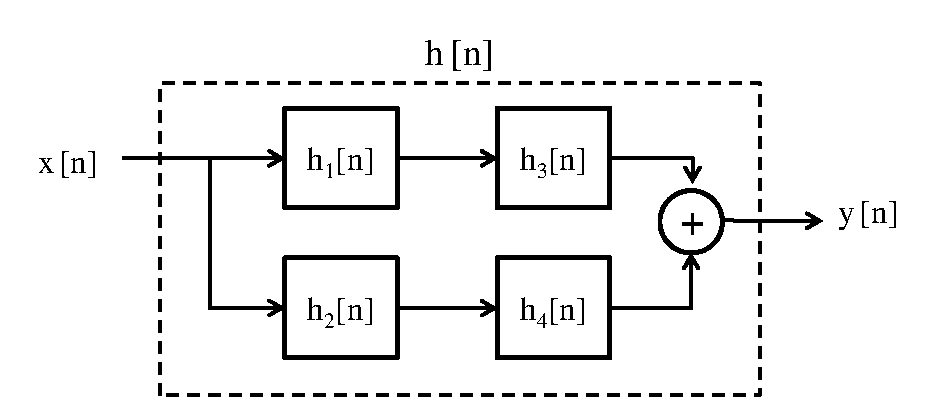
\includegraphics[width=.8\textwidth]{fig1.eps}
\caption{System composed of several sub-systems.}
\label{fig1}
\end{figure}

\vspace{1cm}

\noindent \textbf{4.} (5 points) Given a continuous-time signal $x(t)$ with autocorrelation function $\phi_{xx}(\tau)$, find an expression for the aucorrelation function $\phi_{yy}(\tau)$ of a signal $y(t)$ such that:

\[
y(t) = x(t)+\alpha x(t-\Delta)
\]

\noindent where $\alpha$ and $\Delta$ are constants. Express your answer in terms of $\phi_{xx}(\tau)$.

\vspace{1cm}

\noindent \textbf{5.} (5 points) Justify the fact that, if a discrete-time system is linear and time invariant (LTI), the output of the system to an arbitrary discrete-time input signal can be determined using only the impulse response of the system.  

\end{document}